%\documentclass[draft, 12pt]{article}
\documentclass[12pt]{article}
\usepackage[utf8]{inputenc} % следующие две строки используются для
\usepackage[english,russian]{babel}   % руссификации AmSLaTeX
\usepackage{amsmath,amsfonts,amssymb,euscript,graphicx,wrapfig,multirow}
\usepackage{dsfont}
\inputencoding{utf8}
\textheight=240mm \textwidth=170mm
\hoffset=-17mm % сдвиг влево
\voffset=-17mm % сдвиг вверх

\begin{document}

\noindent УДК 511.95 + 514.112

\begin{center}
\textbf{ОБ ОТЫСКАНИИ ЦЕЛОУДАЛЁННЫХ МНОЖЕСТВ СПЕЦИАЛЬНОГО ВИДА} \\[3mm]
\textbf{Н.~Н.~Авдеев}\\[2mm]
\emph{ВГУ}
\end{center}

Целоудалённым множеством (ЦМ) будем называть такое подмножество $M$ плоскости $\mathbb{R}^2$,
не содержащееся ни в какой прямой,
что расстояние между любыми двумя точками $M$ есть целое число.

Эрдёш [1,2] доказал, что любое ЦМ конечно.
(Доказательство на русском языке можно найти в [3].)

Для ЦМ естественным образом определяется диаметр:
$$
	diam(M) = \max_{A,B\in M} |A-B|,
$$
где $|A-B|$~--- обычное расстояние между $A$ и $B$.

Задача об отыскании ЦМ заданного диаметра и мощности первоначально возникла
в ходе определения минимального диаметра,
которым может обладать множество заданной мощности [4].
Затем, в ходе развития классификации ЦМ и выделения множеств полуобщего и общего положения,
встал вопрос от отыскании ЦМ, обладающих специальными свойствами.


В данной работе описывается отыскание <<необычных>>, в некотором смысле, ЦМ.

Выделяют веерные ЦМ, т.е. ЦМ, лежащие на объединении прямой и некоторой точки.
Именно веерные ЦМ имеют наименьший диаметр среди всех ЦМ мощности от 9 до 122 [5];
однако с помощью веерных ЦМ невозможно построить конструктивную оценку на минимальный диаметр,
которая была бы существенно лучше, чем существующая [4], основанная на содержащихся в окружности ЦМ.
Таким образом, относительно хорошо известны ЦМ, лежащие в объединении точки с прямой или окружности с её центром.
Отыскание таких ЦМ выходит за пределы целей данной работы.

На основе веерного ЦМ характеристики 1 легко строится ЦМ, содержащееся в двух перпендикулярных прямых,
при этом на одной из прямых лежит 2 или 3 точки, на другой~--- все остальные
(точка пересечения прямых может как принадлежать ЦМ, так и не принадлежать ему).
Отыскание ЦМ, содержащихся в паре перпендикулярных прямых и распределённых по этим прямым
<<более равномерно>>, де-факто оказывается чисто алгебраической задачей [6];
наиболее интересным, на взгляд автора, является следующий пример из [6]:
$$
\{
(0,0);
(0,\pm 9282000),
(0,\pm 26822600),
(0,\pm 60386040);
$$
$$
(\pm 7422030,0),
(\pm 8947575, 0),
(\pm 22276800,0),
(\pm 44142336,0)
\}
.
$$

Таким образом, нас будут интересовать все ЦМ, кроме ЦМ, содержащихся:
а) в объединении прямой с точкой, не лежащей на ней (веерные ЦМ);
б) в объединении окружности с её центром;
в) в паре перпендикулярных прямых.

Для отыскания ЦМ используется алгоритм, описанный в [7],
со следующими изменениями.
Во-первых, нахождение ЦМ с заданным диаметром и мощностью не приводит к прекращению процесса поиска.
Во-вторых, в модифицированном алгоритме Брона-Кербоша за начальную клику
принимается не произвольная точка, лежащая за пределами прямой, проходящей через точки,
на которых достигается диаметр, а пара таких точек (если расстояние между точкми пары есть число целое).
Это отсекает значительное количество (но не все) веерных ЦМ.

Все найденные таким алгоритмом ЦМ подвергаются проверке на выполнение одного из условий (а)--(в);
если ни одно из условий не выполнено, информация о ЦМ записывается в файл и строится визуализация найденного ЦМ с помощью gnuplot
[8,9].

Ниже приводятся иллюстрированные примеры найденных ЦМ из числа наиболее интересных.
Для облегчения восприятия применяется запись вида
$\sqrt{p}/q * \{ (x_1,y_1), ...,$ $ (x_n, y_n)  \}$,
означающая, что каждую абсциссу нужно умножить на $1/q$,
а каждую ординату~--- умножить на $\sqrt{p}/q$, т.е.
$$
	\sqrt{p}/q * \{ (x_1,y_1), ..., (x_n, y_n)  \}
	=
	\left\{ \left(\frac{x_1}{q},\frac{y_1\sqrt{p}}{q}\right), ..., \left(\frac{x_n}{q},\frac{y_n\sqrt{p}}{q}\right)  \right\}
	.
$$

Чаще всего из интересующих нас ЦМ встречаются ЦМ, содержащиеся в паре параллельных прямых,
причём на одной из прямых лежит две или три точки.

\begin{itemize}
\setlength{\itemsep}{-1mm}


\item
$\sqrt{35}/{34} * \{ (\pm 289, 0),
%(289 , 0),
(88 , -39),
(-144 , -15),
(-175 , 48),
(-57 , -24),
(57 , 24)\} $
(рис.~\ref{Avdeev_7_17_1538484835387.eps}).
%ЦМ мощности 7, диаметр 17.
На этом ЦМ достигается минимальное значение диаметра для мощности 7,
однако в [4, fig. 1] это ЦМ приведено не было:
примером ЦМ мощности 7 и диаметра 17 послужило другое ЦМ.

\item
$\sqrt{3}/2 * \{
( \pm 56 , 0),
( 14 , 0),
( -34 , 0),
( -10 , 24),
( -21 , 35),
( 35 , -21)
\}
$
(рис.~\ref{Avdeev_7_56_1538484851696.eps}).
ЦМ лежит на двух пересекающихся под острым углом прямых и имеет ось симметрии
~--- биссектрису угла между прямыми.


\begin{figure}[htbp]
	\includegraphics[width=.48\linewidth]{Avdeev_7_17_1538484835387.eps}
	\hfill
	\includegraphics[width=.48\linewidth]{Avdeev_7_56_1538484851696.eps}
	\\
	\parbox{.48\linewidth}{\caption{ЦМ мощности 7, диаметр 17}\label{Avdeev_7_17_1538484835387.eps}}
	\hfill
	\parbox{.48\linewidth}{\caption{ЦМ мощности 7, диаметр 56}\label{Avdeev_7_56_1538484851696.eps}}
\end{figure}

\item
$
\sqrt{39}/8 *
\{
( \pm240 , 0),
( -91 , -15),
( -35 , -55),
( -140 , 20),
( -112 , 0),
( -16 , 0)
\}
$
(рис.~\ref{Avdeev_7_60_1538484853808.eps}).
Ещё один пример с двумя пересекающимися прямыми.

\item
$
\sqrt{7}/2 *
\{
( \pm60 , 0),
( \pm15 , -25),
( \pm33 , -9),
( 0 , -20)
\}
$
(рис.~\ref{Avdeev_7_60_1538484854748.eps}).
Прямые не перпендикулярны, как может показаться.

\begin{figure}[htbp]
	\includegraphics[width=.48\linewidth]{Avdeev_7_60_1538484853808.eps}
	\hfill
	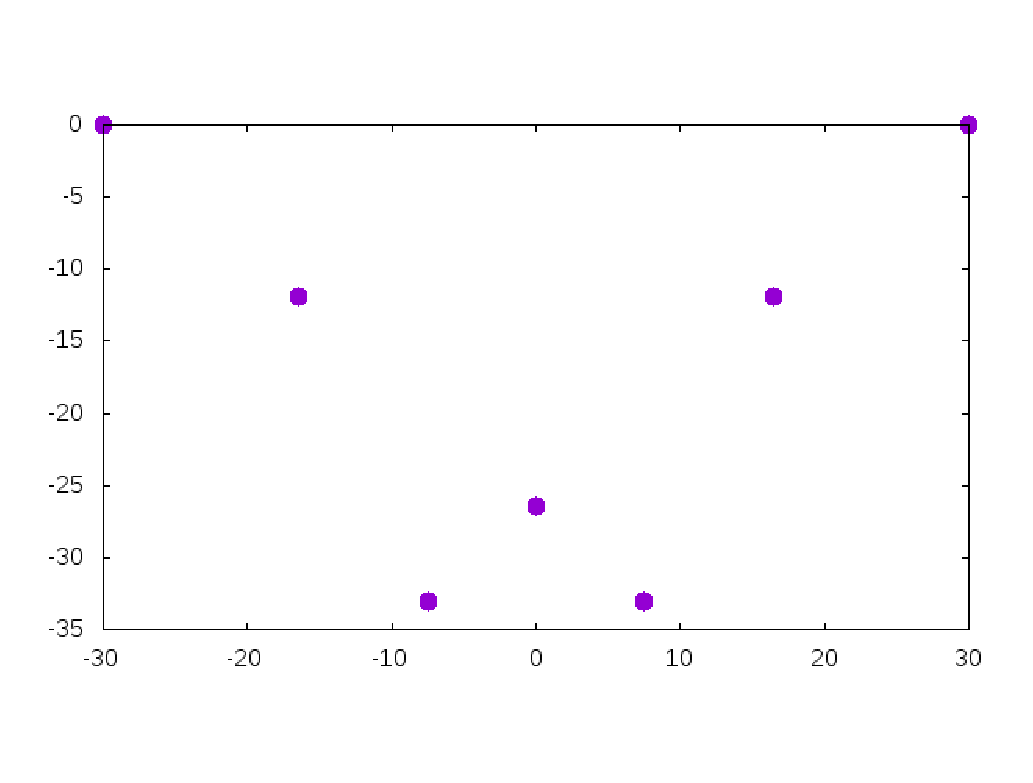
\includegraphics[width=.48\linewidth]{Avdeev_7_60_1538484854748.eps}
	\\
	\parbox{.48\linewidth}{\caption{ЦМ мощности 7, диаметр 60}\label{Avdeev_7_60_1538484853808.eps}}
	\hfill
	\parbox{.48\linewidth}{\caption{ЦМ мощности 7, диаметр 60}\label{Avdeev_7_60_1538484854748.eps}}
\end{figure}

\item
$
\sqrt{7}/2 *
\{
( \pm64 , 0),
( \pm45 , 15),
( \pm19 , 15),
( 0 , 0)
\}
$
(рис.~\ref{Avdeev_7_64_1538484861024.eps}).

\item
$
\sqrt{3}/2 *
\{
( \pm75 , 0),
( 29 , -24),
( -35 , 40),
( 40 , -35),
( 5 , 0),
( 53 , 0)
\}
$
(рис.~\ref{Avdeev_7_75_1538484880810.eps}).


\begin{figure}[htbp]
	\includegraphics[width=.48\linewidth]{Avdeev_7_64_1538484861024.eps}
	\hfill
	\includegraphics[width=.48\linewidth]{Avdeev_7_75_1538484880810.eps}
	\\
	\parbox{.48\linewidth}{\caption{ЦМ мощности 7, диаметр 64}\label{Avdeev_7_64_1538484861024.eps}}
	\hfill
	\parbox{.48\linewidth}{\caption{ЦМ мощности 7, диаметр 75}\label{Avdeev_7_75_1538484880810.eps}}
\end{figure}

\item
$
\sqrt{15}/2 *
\{
( \pm77 , 0),
( 0 , 13),
( \pm28 , -15),
( \pm11 , 24)
\}
$
(рис.~\ref{Avdeev_7_77_1538484885363.eps}).

\item
$
\sqrt{15}/4 *
\{
( \pm156 , 0),
( -9 , -45),
( -145 , 11),
( 112 , -12),
( 128 , -28),
( 68 , 32)
\}
$
(рис.~\ref{Avdeev_7_78_1538484891588.eps}).


\begin{figure}[htbp]
	\includegraphics[width=.48\linewidth]{Avdeev_7_77_1538484885363.eps}
	\hfill
	\includegraphics[width=.48\linewidth]{Avdeev_7_78_1538484891588.eps}
	\\
	\parbox{.48\linewidth}{\caption{ЦМ мощности 7, диаметр 77}\label{Avdeev_7_77_1538484885363.eps}}
	\hfill
	\parbox{.48\linewidth}{\caption{ЦМ мощности 7, диаметр 78}\label{Avdeev_7_78_1538484891588.eps}}
\end{figure}


\item
$
\sqrt{455}/2 *
\{
( \pm87 , 0),
( \pm64 , -3),
( 0 , -3),
( \pm23 , 0)
\}
$
(рис.~\ref{Avdeev_7_87_1538484975645.eps}).

\item
$
\sqrt{15}/4 *
\{
( \pm180 , 0),
( 135 , 45),
( -33 , 21),
( 44 , 32),
( 76 , 0),
( -12 , 0)
\}
$
(рис.~\ref{Avdeev_7_90_1538485007759.eps}).

\begin{figure}[htbp]
	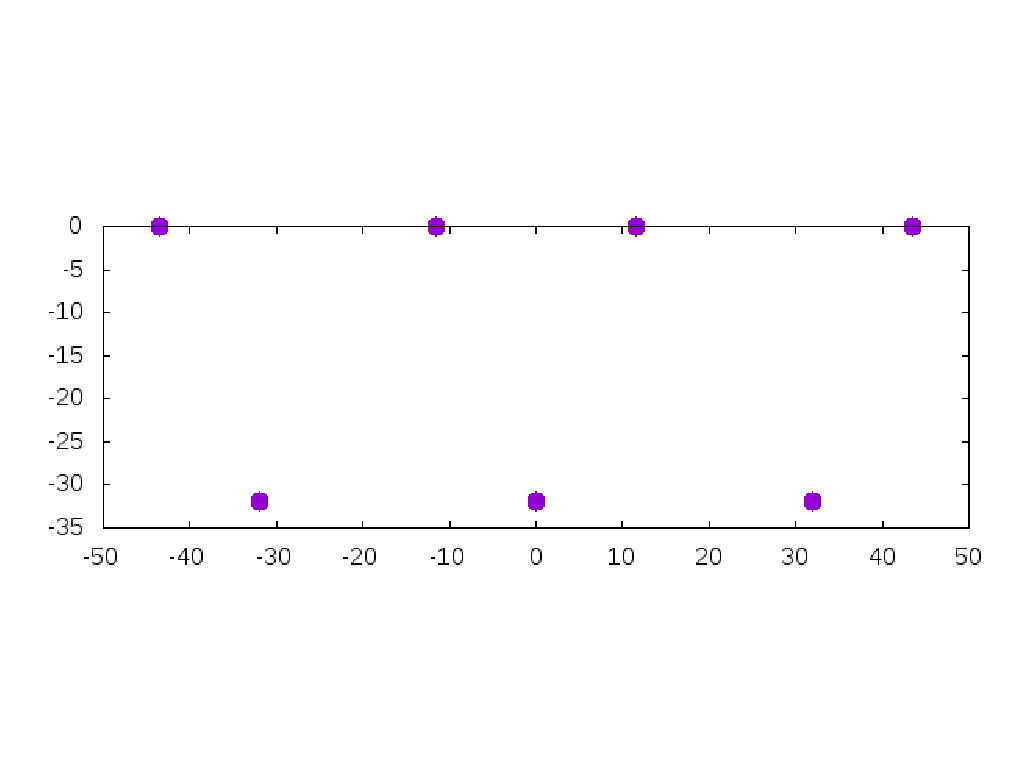
\includegraphics[width=.48\linewidth]{Avdeev_7_87_1538484975645.eps}
	\hfill
	\includegraphics[width=.48\linewidth]{Avdeev_7_90_1538485007759.eps}
	\\
	\parbox{.48\linewidth}{\caption{ЦМ мощности 7, диаметр 87}\label{Avdeev_7_87_1538484975645.eps}}
	\hfill
	\parbox{.48\linewidth}{\caption{ЦМ мощности 7, диаметр 90}\label{Avdeev_7_90_1538485007759.eps}}
\end{figure}



\item
$
\sqrt{35}/1 *
\{
( \pm27 , 8),
( 0 , 8),
( \pm46 , 0),
( \pm19 , 0)
\}
$
(рис.~\ref{Avdeev_7_92_1538485051452.eps}).

\item
$
\sqrt{15}/2 *
\{
( -95 , 0),
( 95 , 0),
( -84 , -11),
( -52 , 21),
( -7 , -24),
( -73 , 0),
( -31 , 0)
\}
$
(рис.~\ref{Avdeev_7_95_1538485087074.eps}).

\begin{figure}[htbp]
	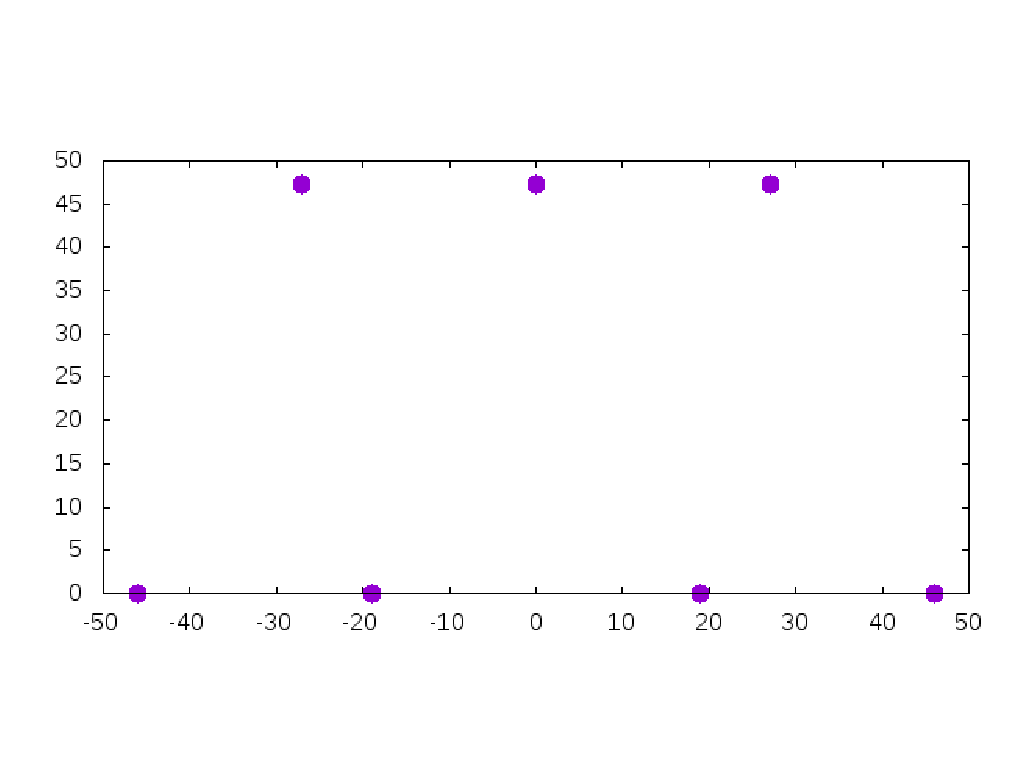
\includegraphics[width=.48\linewidth]{Avdeev_7_92_1538485051452.eps}
	\hfill
	\includegraphics[width=.48\linewidth]{Avdeev_7_95_1538485087074.eps}
	\\
	\parbox{.48\linewidth}{\caption{ЦМ мощности 7, диаметр 92}\label{Avdeev_7_92_1538485051452.eps}}
	\hfill
	\parbox{.48\linewidth}{\caption{ЦМ мощности 7, диаметр 95}\label{Avdeev_7_95_1538485087074.eps}}
\end{figure}


\item
$
\sqrt{15}/8 *
\{
( -384 , 0),
( 384 , 0),
( -100 , -28),
( 155 , 77),
( -253 , -91),
( -32 , 0),
( 96 , 0)
\}
$
(рис.~\ref{Avdeev_7_96_1538485207044.eps}).


\item
$
\sqrt{91}/2 *
\{
( \pm99 , 0),
( 0 , 17),
( \pm75 , -8),
( \pm24 , 9)
\}
$
(рис.~\ref{Avdeev_7_99_1538485281307.eps}).


\begin{figure}[htbp]
	\includegraphics[width=.48\linewidth]{Avdeev_7_96_1538485207044.eps}
	\hfill
	\includegraphics[width=.48\linewidth]{Avdeev_7_99_1538485281307.eps}
	\\
	\parbox{.48\linewidth}{\caption{ЦМ мощности 7, диаметр 96}\label{Avdeev_7_96_1538485207044.eps}}
	\hfill
	\parbox{.48\linewidth}{\caption{ЦМ мощности 7, диаметр 99}\label{Avdeev_7_99_1538485281307.eps}}
\end{figure}


\item
$
\sqrt{91}/2 *
\{
( \pm99 , 0),
( 0 , 17),
( \pm24 , 9),
( 75 , -8),
( 51 , 0)
\}
$
(рис.~\ref{Avdeev_7_99_1538485281335.eps}).

\item
$
\sqrt{91}/2 *
\{
( \pm99 , 0),
( 0 , 17),
( \pm24 , 9),
( \pm51 , 0)
\}
$
(рис.~\ref{Avdeev_7_99_1538485281337.eps}).


\begin{figure}[htbp]
	\includegraphics[width=.48\linewidth]{Avdeev_7_99_1538485281335.eps}
	\hfill
	\includegraphics[width=.48\linewidth]{Avdeev_7_99_1538485281337.eps}
	\\
	\parbox{.48\linewidth}{\caption{ЦМ мощности 7, диаметр 99}\label{Avdeev_7_99_1538485281335.eps}}
	\hfill
	\parbox{.48\linewidth}{\caption{ЦМ мощности 7, диаметр 99}\label{Avdeev_7_99_1538485281337.eps}}
\end{figure}



\item
$
\sqrt{3003}/82 *
\{
( \pm5043 , 0),
( 3640 , 23),
( 1200 , 63),
( 2277 , -120),
( -163 , -80),
( 2603 , 40),
$ \\ $
( -2603 , -40)
\}
$
(рис.~\ref{Avdeev_8_123_1538485378899.eps}).
ЦМ лежит на двух прямых, по 4 точки на каждой.

\item
$
\sqrt{3003}/82 *
\{
( \pm5043 , 0),
( -1240 , -103),
( 3640 , -23),
( 1200 , -63),
( -163 , 80),
( 163 , -80),
$ \\ $
( -2603 , 40)
\}
$
(рис.~\ref{Avdeev_8_123_1538485378698.eps}).
ЦМ лежит на двух прямых, 3 точки на одной и 5 на другой.


\begin{figure}[htbp]
	\includegraphics[width=.48\linewidth]{Avdeev_8_123_1538485378899.eps}
	\hfill
	\includegraphics[width=.48\linewidth]{Avdeev_8_123_1538485378698.eps}
	\\
	\parbox{.48\linewidth}{\caption{ЦМ мощности 8, диаметр 123}\label{Avdeev_8_123_1538485378899.eps}}
	\hfill
	\parbox{.48\linewidth}{\caption{ЦМ мощности 8, диаметр 123}\label{Avdeev_8_123_1538485378698.eps}}
\end{figure}


\item
$
\sqrt{210}/73 *
\{
( \pm5329 , 0),
( -3783 , -272),
( 3922 , -42),
( 1309 , -120),
( -2376 , -230),
$ \\ $
( 237 , -152),
( 3515 , 264)
\}
$
(рис.~\ref{Avdeev_8_146_1538486493354.eps}).

\item
$
\sqrt{2}/27 *
\{
( \pm2187 , 0),
( 1309 , 1520),
( 899 , -560),
( 623 , -680),
( -665 , -1240),
( 1428 , -330),
$ \\ $
( 94 , -910)
\}
$
(рис.~\ref{Avdeev_8_162_1538488466583.eps}).

\begin{figure}[htbp]
	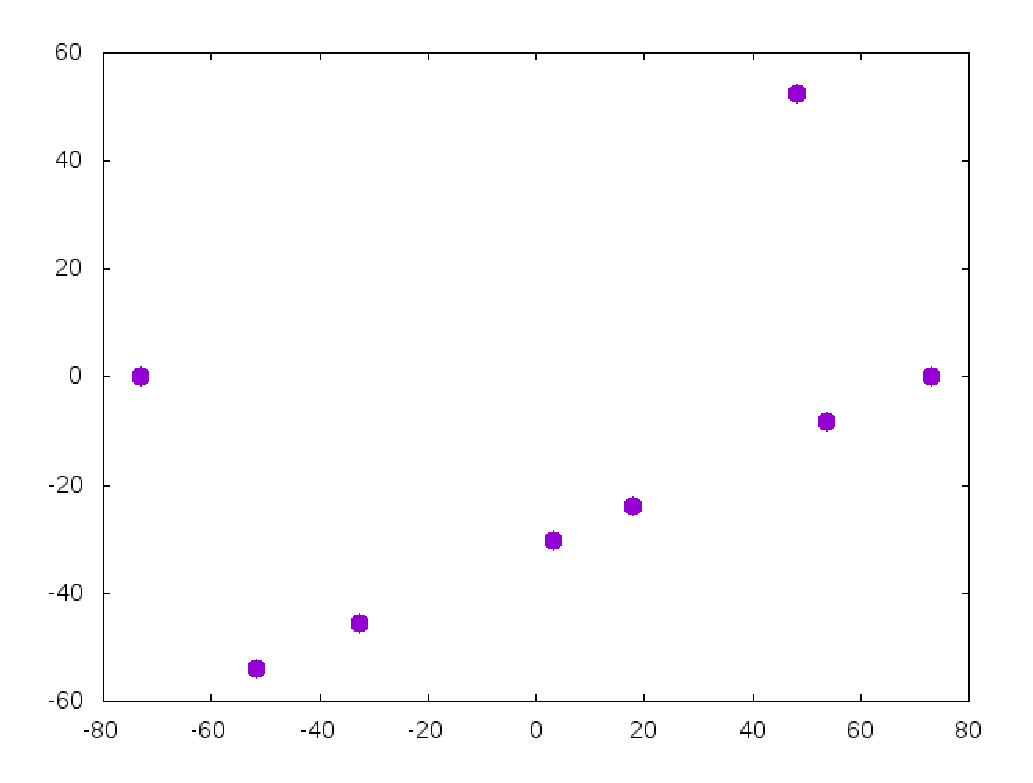
\includegraphics[width=.48\linewidth]{Avdeev_8_146_1538486493354.eps}
	\hfill
	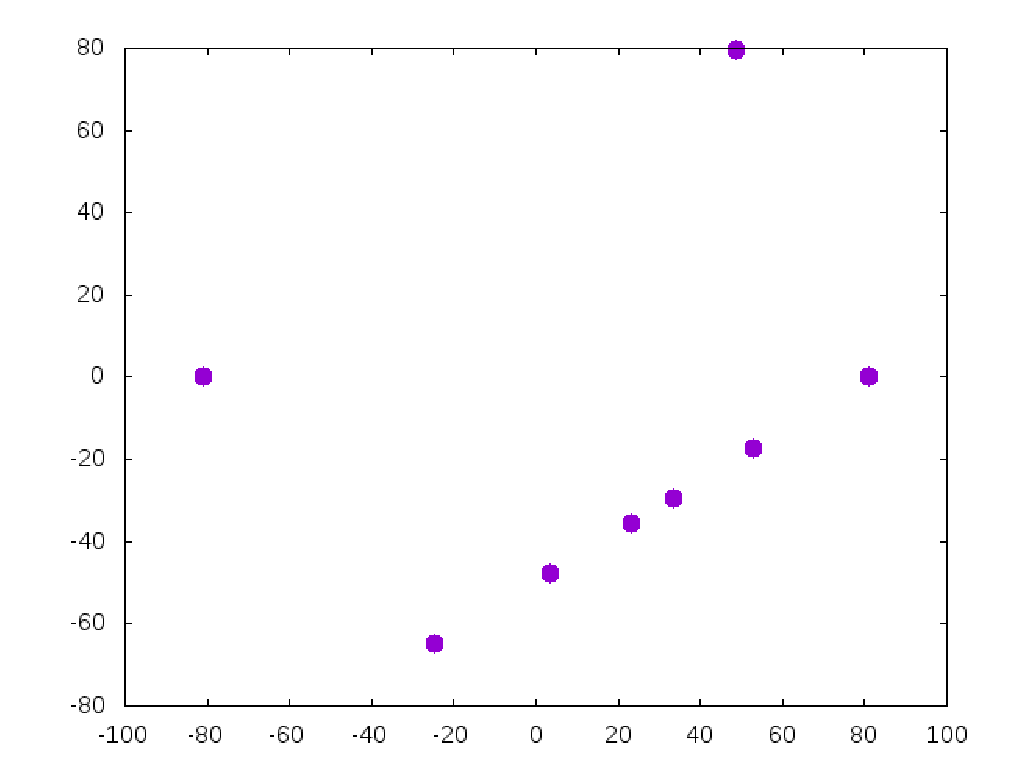
\includegraphics[width=.48\linewidth]{Avdeev_8_162_1538488466583.eps}
	\\
	\parbox{.48\linewidth}{\caption{ЦМ мощности 8, диаметр 146}\label{Avdeev_8_146_1538486493354.eps}}
	\hfill
	\parbox{.48\linewidth}{\caption{ЦМ мощности 8, диаметр 162}\label{Avdeev_8_162_1538488466583.eps}}
\end{figure}


\item
$
\sqrt{1}/1 *
\{
( \pm84 , 0),
( \pm24 , 45),
( 0 , 63),
( 0 , 13),
( 0 , 35),
( 0 , 0)
\}
$
(рис.~\ref{Avdeev_8_168_1538490487450.eps}).
ЦМ лежит на целочисленной решётке.

\item
$
\sqrt{231}/2 *
\{
( \pm171 , 0),
( \pm96 , 9),
( \pm125 , -8),
( \pm21 , 0)
\}
$
(рис.~\ref{Avdeev_8_171_1538491142044.eps}).


\begin{figure}[htbp]
	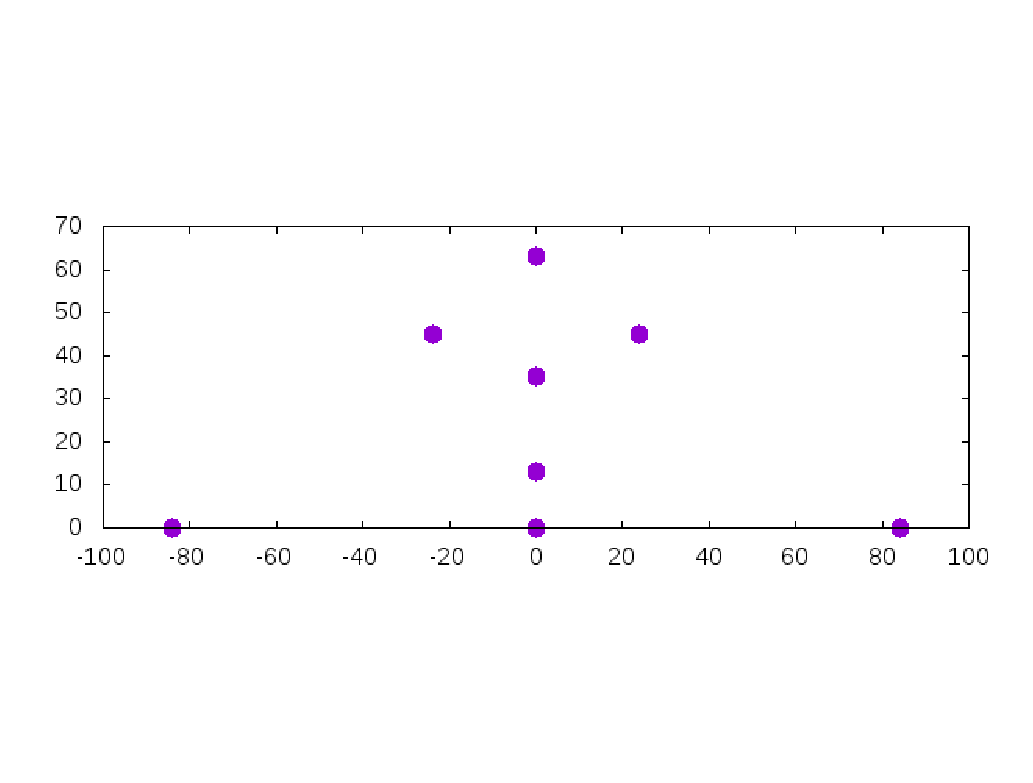
\includegraphics[width=.48\linewidth]{Avdeev_8_168_1538490487450.eps}
	\hfill
	\includegraphics[width=.48\linewidth]{Avdeev_8_171_1538491142044.eps}
	\\
	\parbox{.48\linewidth}{\caption{ЦМ мощности 8, диаметр 168}\label{Avdeev_8_168_1538490487450.eps}}
	\hfill
	\parbox{.48\linewidth}{\caption{ЦМ мощности 8, диаметр 171}\label{Avdeev_8_171_1538491142044.eps}}
\end{figure}






\item
$
\sqrt{3003}/82 *
\{
( \pm5043 , 0),
( -163 , -80),
( 163 , 80),
( 2603 , 40),
( -2603 , -40),
$ \\ $
( 1240 , -103),
( -1200 , -63),
( -3640 , -23)
\}
$
(рис.~\ref{Avdeev_9_123_1538485102263.eps}).


\item
$
\sqrt{210}/107 *
\{
( \pm11449 , 0),
( -3795 , -296),
( -7812 , -374),
( 4033 , -144),
( -9975 , -416),
$ \\ $
( 1870 , -186),
( -2147 , -264),
( 2147 , 264)
\}
$
(рис.~\ref{Avdeev_9_214_1538495187150.eps}).

\begin{figure}[htbp]
	\includegraphics[width=.48\linewidth]{Avdeev_9_123_1538485102263.eps}
	\hfill
	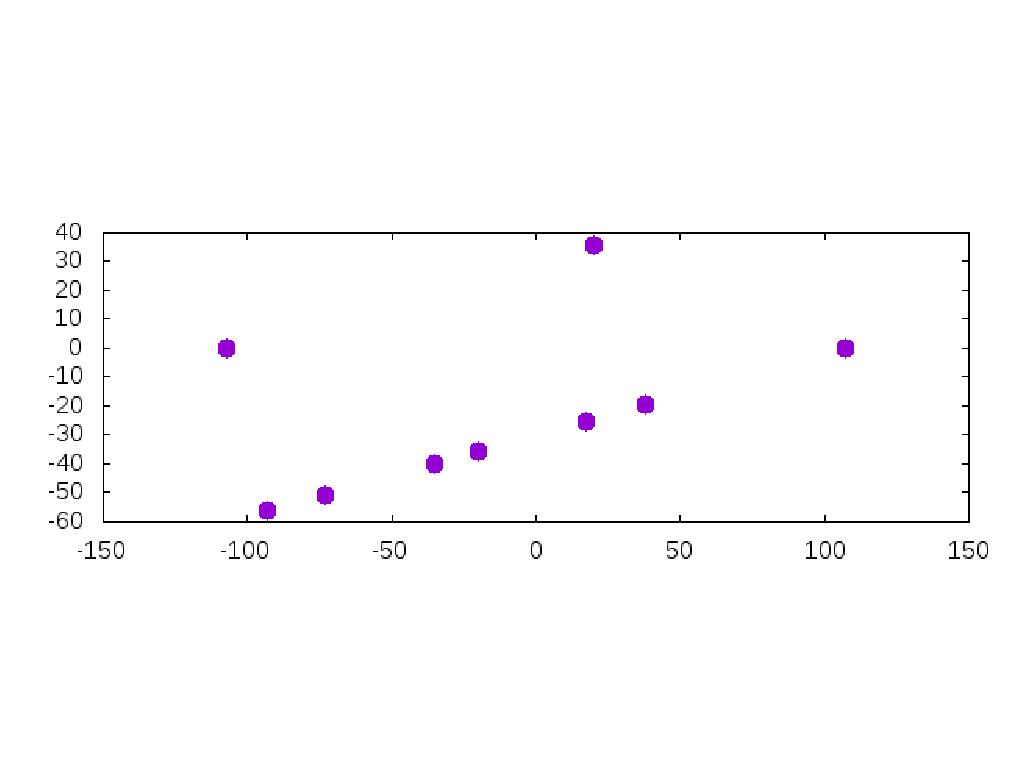
\includegraphics[width=.48\linewidth]{Avdeev_9_214_1538495187150.eps}
	\\
	\parbox{.48\linewidth}{\caption{ЦМ мощности 9, диаметр 123}\label{Avdeev_9_123_1538485102263.eps}}
	\hfill
	\parbox{.48\linewidth}{\caption{ЦМ мощности 9, диаметр 214}\label{Avdeev_9_214_1538495187150.eps}}
\end{figure}





%\begin{figure}[htbp]
%	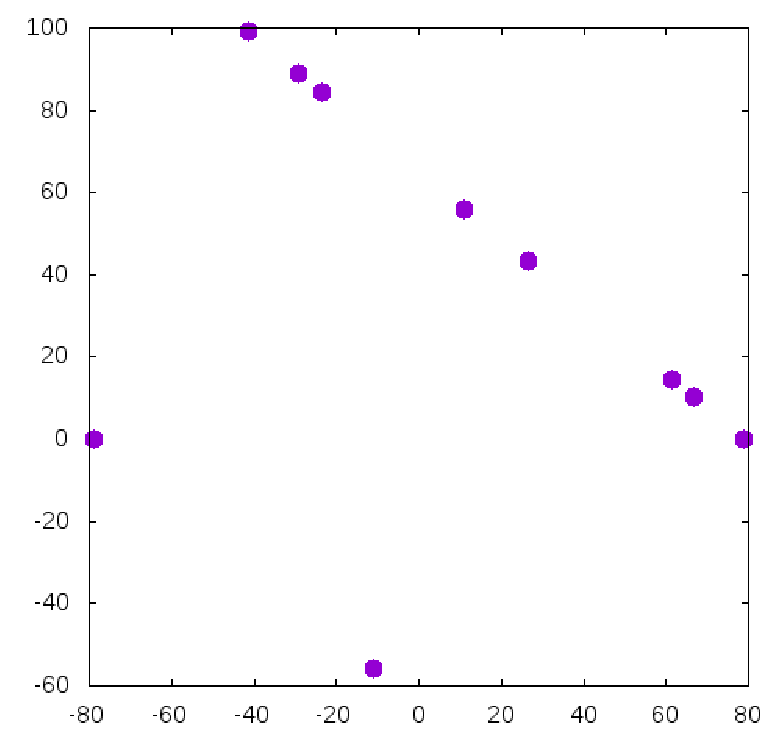
\includegraphics[width=.48\linewidth]{Avdeev_10_158_1538485325776.eps}
%	\hfill
%	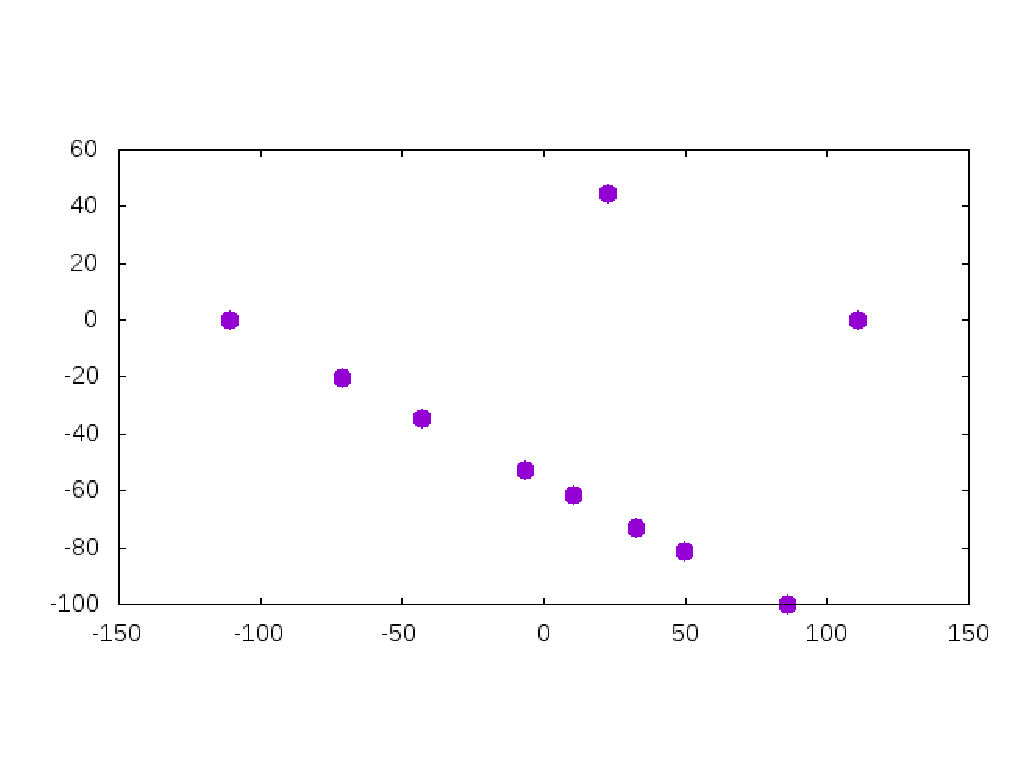
\includegraphics[width=.48\linewidth]{Avdeev_10_222_1538488624864.eps}
%	\\
%	\parbox{.48\linewidth}{\caption{ЦМ мощности 10, диаметр 158}\label{Avdeev_10_158_1538485325776.eps}}
%	\hfill
%	\parbox{.48\linewidth}{\caption{ЦМ мощности 10, диаметр 222}\label{Avdeev_10_222_1538488624864.eps}}
%\end{figure}

\end{itemize}

{\small Работа выполнена в Воронежском университете при поддержке РНФ, грант 16-11-10125.}


\bigskip\centerline{\bf Литература}



1.	\emph{Anning~N. H., Erd\"{o}s~P.}
	Integral distances // Bulletin of the American Mathematical
	Society. --- 1945. --- Т. 51, No 8. --- С. 598---600.

2.	\emph{Erd\"{o}s~P.} Integral distances // Bulletin of the
	American Mathematical Society. --- 1945. --- Т. 51, No 12. --- С. 996.

3.	\emph{Авдеев Н. Н., Семенов Е. М.}
	Множества точек с целочисленными расстояниями на плоскости и в евклидовом пространстве
	//
	Сборник материалов XIV Владикавказской молодежной математической Школы-конференции.
	--- 2018 --- (в печати)

4.	\emph{Harborth~H.,
	Kemnitz~A.,
	M\"{o}ller~M.}
	An upper bound for the minimum diameter of integral point sets
	/\!/ Discrete \& Computational Geometry. --- 1993. --- Т. 9, No 4.
	--- С. 427---432.

5.	\emph{Kurz~S., Wassermann~A.}
	On the minimum diameter of plane integral point sets /\!/ arXiv
	preprint arXiv:0804.1307. --- 2008.

6.	\emph{Guy~R.} Unsolved problems in number theory. Т.
	1. --- Springer Science \& Business Media, 2013.

7.	\emph{Авдеев~Н. Н.} Об отыскании множеств точек на
	плоскости с целочисленными расстояниями /\!/ Математическое
	и компьютерное моделирование, информационные технологии
	управления: сб. тр. Школы для студентов, аспирантов и
	молодых ученых <<МКМИТУ-2016>>. --- 2016. --- С. 15---19.

8.	\emph{Балдин Е.} Gnuplot. Графики заказывали? //Системный администратор. – 2007. – №. 4. – С. 72-77.

9.	\emph{Алексеев Е. Р., Демин П. А., Костюк Д. А.} Возможности графического вывода результатов в последовательных и
	параллельных кроссплатформенных вычислительных приложениях на Фортране и С(С++) // Advanced science, 2017, №3.



{\bf Авдеев Николай Николаевич},
бакалавр математики, магистрант кафедры функционального анализа и операторных уравнений математического факультета
ФГБОУ ВО <<Воронежский государственный университет>>, г. Воронеж.

E-mail: avdeev@math.vsu.ru, nickkolok@mail.ru

Научный руководитель: Семенов Евгений Михайлович.

\end{document}

